\documentclass[preprint,12pt,aps,pra,showkeys,amsmath,amssymb,superscriptaddress,floatfix]{revtex4-2}
\usepackage[T1]{fontenc}
\usepackage[utf8]{inputenc}
\usepackage{amsmath,amssymb,amsthm,mathtools,mathrsfs}
\usepackage{microtype,booktabs,enumitem}
\usepackage{xcolor,tikz,etoolbox}
\usepackage[skins,breakable]{tcolorbox}
\usepackage{needspace}
% Keep diagram geometry independent of REVTeX preprint body spacing.
\AtBeginEnvironment{tikzpicture}{\linespread{1}\selectfont}
\usetikzlibrary{arrows.meta,positioning,calc,fit,decorations.pathreplacing}
\usepackage{graphicx}
\usepackage{hyperref}

\definecolor{MMBlue}{RGB}{0,82,155}
\definecolor{MMOrange}{RGB}{200,80,0}
\tikzset{
 mmnode/.style={draw=MMBlue,rounded corners=2pt,fill=MMBlue!4,align=left,execute at begin node={\raggedright},text width=5cm,font=\fontsize{10}{12}\selectfont,inner sep=6pt},
 mmimport/.style={mmnode,draw=black!65,fill=black!4},
 mmcandidate/.style={mmnode,draw=MMOrange,dashed,fill=MMOrange!5},
 mmrejected/.style={mmnode,draw=black,densely dotted,fill=black!8},
 mmproof/.style={->,thick,MMBlue},
 mmflow/.style={->,semithick,black!70},
 mmrepair/.style={->,dashed,thick,MMOrange},
 mmcandidatearrow/.style={->,dashed,semithick,MMOrange},
 mmnote/.style={font=\scriptsize,fill=white,inner sep=2pt,align=center}}

\usepackage[section]{placeins}
\setlength{\emergencystretch}{3em}
\setlist{itemsep=3pt,topsep=4pt}
\newtheorem{theorem}{Theorem}[section]
\newtheorem{proposition}[theorem]{Proposition}
\newtheorem{lemma}[theorem]{Lemma}
\newtheorem{corollary}[theorem]{Corollary}
\theoremstyle{definition}
\newtheorem{definition}[theorem]{Definition}
\newtheorem{example}[theorem]{Example}
\theoremstyle{remark}
\newtheorem{remark}[theorem]{Remark}
% Avoid isolated statement headings and single-line paragraph fragments.
\BeforeBeginEnvironment{theorem}{\Needspace{6\baselineskip}}
\BeforeBeginEnvironment{definition}{\Needspace{5\baselineskip}}
\BeforeBeginEnvironment{proposition}{\Needspace{5\baselineskip}}
\BeforeBeginEnvironment{lemma}{\Needspace{5\baselineskip}}
\BeforeBeginEnvironment{corollary}{\Needspace{5\baselineskip}}
\clubpenalty=5000
\widowpenalty=5000
\newcommand{\R}{\mathbb R}\newcommand{\Z}{\mathbb Z}\newcommand{\N}{\mathbb N}
\newcommand{\Pa}{\operatorname{Pa}}\newcommand{\Desc}{\operatorname{Desc}}
\newcommand{\cl}{\operatorname{cl}}\newcommand{\cost}{\operatorname{cost}}
\newcommand{\status}{\operatorname{status}}
% Faculty cards: a visual rail groups the five faculties within one agent.
% The rail has no arrowhead and does not represent a proof dependency.
\newcommand{\mmfacultybadge}[1]{%
 \node[circle,draw=MMBlue,line width=1pt,fill=white,
 minimum size=7mm,inner sep=0pt,font=\sffamily\small\bfseries,text=MMBlue]
 at ([xshift=15pt,yshift=-15pt]frame.north west) {#1};}
\newcommand{\mmfacultyrail}{%
 \draw[MMBlue!80,line width=1pt]
 ([xshift=15pt,yshift=2pt]frame.north west)--
 ([xshift=15pt,yshift=-2pt]frame.south west);}
\newtcolorbox{mmfacultybox}[2]{enhanced,breakable,
 colback=MMBlue!4,colframe=MMBlue!4,boxrule=0pt,arc=3pt,
 left=39pt,right=9pt,top=4pt,bottom=4pt,
 before skip=2pt,after skip=2pt,
 fontupper=\small\linespread{1.1}\selectfont,
 overlay unbroken={\mmfacultyrail\mmfacultybadge{#1}},
 overlay first={\mmfacultyrail\mmfacultybadge{#1}},
 overlay middle={\mmfacultyrail},overlay last={\mmfacultyrail}}
\newcommand{\mmfaculty}[3]{%
 \begin{mmfacultybox}{#1}{#2}
 {\sffamily\bfseries\color{MMBlue}#2}\par\smallskip #3
 \end{mmfacultybox}}
\newcommand{\agent}[9]{%
 \Needspace{8\baselineskip}
 \subsubsection{#1}
 \noindent\textbf{Object.} #2\par
 \noindent\textbf{Role.} #3\par\smallskip
 \mmfaculty{E}{Ego}{#4}
 \mmfaculty{M}{Memory}{#5}
 \mmfaculty{I}{Intellect}{#6}
 \mmfaculty{S}{Sense}{#7}
 \mmfaculty{A}{Action}{#8}
 \smallskip\noindent #9\par}

\usepackage{longtable,array,calc}
\providecommand{\tightlist}{\setlength{\itemsep}{2pt}\setlength{\parskip}{0pt}}
\makeatletter
\def\frontmatter@abstract@produce{\par\addvspace{\frontmatter@preabstractspace}%
\begingroup\prep@absbox\unvbox\absbox\post@absbox\endgroup
\addvspace{\frontmatter@postabstractspace}}
\makeatother
\newcommand{\field}[2]{\par\smallskip\noindent\textbf{#1.} #2\par}
\setlength{\emergencystretch}{5em}
\AtBeginEnvironment{verbatim}{\small\linespread{1.0}\selectfont}


\hypersetup{colorlinks=true,linkcolor=MMBlue,urlcolor=MMBlue,pdfauthor={Dibakar Sigdel}}

\begin{document}

\title{Strong Law for IID Variables with a Finite Fourth Moment\\[4pt]\large An End-to-End Meta-Math Walkthrough}

\author{Dibakar Sigdel}

\affiliation{Mindverse Computing LLC, Lynnwood, WA 98087, USA}

\date{October 2026}

\begin{abstract}

The fourth moment supplies a summable \(n^{-2}\) deviation bound. A
countable collection of tolerances then upgrades eventual control to
almost sure convergence. The report presents the target theorem,
declared imports, a dependency graph, five-faculty node contracts, a
continuous proof, a worked example, and a hypothesis-repair audit. It is
an authored mathematical exposition, not a deployed-agent transcript or
a formal proof-assistant certificate.

\end{abstract}\maketitle\linespread{1.12}\selectfont

\noindent\textbf{PS-02 / Probability and Stochastic Processes / Report v1}

\section{Target and import contract}

\begin{theorem}

Let \((X_n)_{n\ge1}\) be independent identically distributed real random
variables with \(\mathbb E|X_1|^4<\infty\) and mean \(\mu\). Prove
\(n^{-1}\sum_{j=1}^n X_j\to\mu\) almost surely. This is the
finite-fourth-moment version, not the optimal integrability form of the
strong law.

\end{theorem}

\subsection{Foundations and permitted imports}

Import PS-01(i): summable event probabilities imply only finitely many
occurrences almost surely. Use linearity of expectation, factorization
of expectations of independent integrable products, and Markov's
inequality for nonnegative \(Z\): \(\mathbb P(Z>a)\le\mathbb EZ/a\) for
\(a>0\), obtained by \(Z\ge a1_{\{Z>a\}}\) and integration. Lower
moments are finite by Hölder on a probability space. Centering preserves
a finite fourth moment via \(|x-y|^4\le8(|x|^4+|y|^4)\).

\clearpage\section{Node interaction workflow}

\begin{center}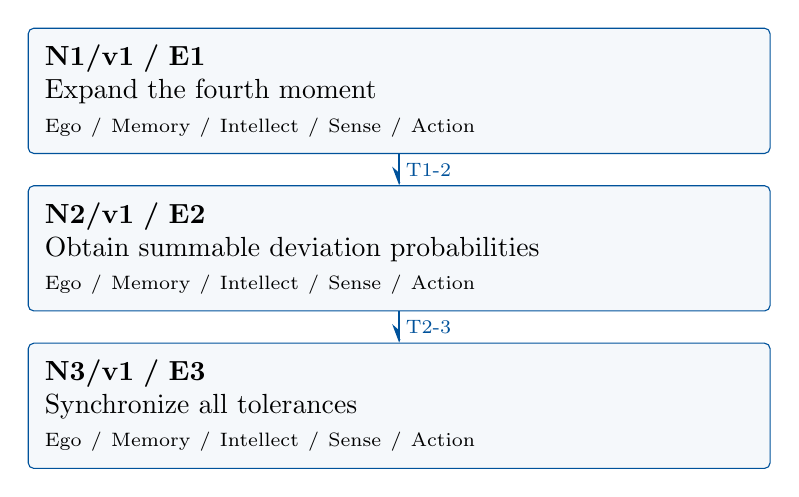
\begin{tikzpicture}[>=Stealth,x=1cm,y=1cm]

\node[mmnode,text width=9cm,minimum height=1.25cm] (N1) at (0,0.0) {\textbf{N1/v1 / E1}\\Expand the fourth moment\\{\scriptsize Ego / Memory / Intellect / Sense / Action}};

\node[mmnode,text width=9cm,minimum height=1.25cm] (N2) at (0,-2.0) {\textbf{N2/v1 / E2}\\Obtain summable deviation probabilities\\{\scriptsize Ego / Memory / Intellect / Sense / Action}};

\node[mmnode,text width=9cm,minimum height=1.25cm] (N3) at (0,-4.0) {\textbf{N3/v1 / E3}\\Synchronize all tolerances\\{\scriptsize Ego / Memory / Intellect / Sense / Action}};

\draw[mmproof] (N1.south) -- node[mmnote,right] {T1-2} (N2.north);

\draw[mmproof] (N2.south) -- node[mmnote,right] {T2-3} (N3.north);

\end{tikzpicture}\end{center}

Each box is one mathematical agent containing all five faculties. Blue
arrows carry the versioned exports listed below. The layout gives a
reading order; only drawn arrows assert dependencies. Diagnostic repair
is separate from the proof DAG.

\subsection{Versioned evidence-transfer ledger}

\begingroup\small\linespread{1.05}\selectfont

\Needspace{5\baselineskip}\field{T1-2: N1/E1/v1 to N2}{\(\mathbb ES_n^4=n m_4+3n(n-1)\sigma^4\).}

\field{Receiving activity}{N2.1}

\field{Compatibility}{E1/v1 and any fixed \(\varepsilon>0\). Check: The bound must be summable
in \(n\); a variance-based \(1/n\) bound is insufficient for this direct
argument.}

\Needspace{5\baselineskip}\field{T2-3: N2/E2/v1 to N3}{\(\sum_n\mathbb P(|S_n/n|>\varepsilon)<\infty\).}

\field{Receiving activity}{N3.1}

\field{Compatibility}{E2/v1 for each \(\varepsilon=1/r\), \(r\in\mathbb N\). Check: An
uncountable intersection of probability-one events is not justified by
countable additivity.}

\endgroup

\clearpage\section{Agent roles and five-faculty activities}\begingroup\small\linespread{1.05}\selectfont\setlist{itemsep=1pt,topsep=2pt}

\subsection{N1/v1: Expand the fourth moment}

\field{Object and role}{Classify the index multiplicities in the fourth-power expansion and use
centering to eliminate singleton factors. \textbf{Local obligation:}
\(\mathbb ES_n^4=n m_4+3n(n-1)\sigma^4\).}

\field{Inputs}{\(Y_j=X_j-\mu\), \(S_n=\sum_{j=1}^nY_j\), \(\sigma^2=\mathbb EY_1^2\),
and \(m_4=\mathbb EY_1^4\).}

\mmfaculty{E}{Ego}{Publish E1/v1 only after establishing this obligation:
\(\mathbb ES_n^4=n m_4+3n(n-1)\sigma^4\).}

\mmfaculty{M}{Memory}{\(Y_j=X_j-\mu\), \(S_n=\sum_{j=1}^nY_j\), \(\sigma^2=\mathbb EY_1^2\),
and \(m_4=\mathbb EY_1^4\). Retain the stated assumptions and import
versions.}

\mmfaculty{I}{Intellect}{Classify the index multiplicities in the fourth-power expansion and use
centering to eliminate singleton factors.}

\mmfaculty{S}{Sense}{Independence and zero means eliminate terms with any index appearing
exactly once; pair terms have combinatorial coefficient six.}

\mmfaculty{A}{Action}{Carry out activities N1.1--N1.2 below, retaining each calculation and
construction as evidence.}

\smallskip\noindent\textbf{Numbered mathematical activities}

\begin{enumerate}[label=N1.\arabic*,leftmargin=3.4em]

\item Expand \((\sum_jY_j)^4\). If an index occurs once in a term,
independence factors out its zero mean, so that term has expectation
zero. The surviving terms are the \(n\) fourth powers \(Y_j^4\) and
terms with two distinct indices each repeated twice.

\item For each unordered pair \(i<j\), there are \(4!/(2!2!)=6\) placements,
and the expectation of \(Y_i^2Y_j^2\) is \(\sigma^4\). Thus the total is
\(n m_4+6\binom n2\sigma^4=n m_4+3n(n-1)\sigma^4\). All terms are
integrable by the declared moment and independence.

\end{enumerate}

\field{Export E1/v1}{\(\mathbb ES_n^4=n m_4+3n(n-1)\sigma^4\).}

\field{Acceptance gate}{Independence and zero means eliminate terms with any index appearing
exactly once; pair terms have combinatorial coefficient six.}

\field{Targeted repair}{If all cross terms are discarded, restore the paired-index terms;
centering kills singletons, not products of squares. Withhold this
export and recheck its descendants after a versioned correction.}

\clearpage

\subsection{N2/v1: Obtain summable deviation probabilities}

\field{Object and role}{Apply Markov to the fourth power of the centered sample mean.
\textbf{Local obligation:}
\(\sum_n\mathbb P(|S_n/n|>\varepsilon)<\infty\).}

\field{Inputs}{E1/v1 and any fixed \(\varepsilon>0\). Incoming proof exports: E1/v1 at
N2.1.}

\mmfaculty{E}{Ego}{Publish E2/v1 only after establishing this obligation:
\(\sum_n\mathbb P(|S_n/n|>\varepsilon)<\infty\).}

\mmfaculty{M}{Memory}{E1/v1 and any fixed \(\varepsilon>0\). Incoming proof exports: E1/v1 at
N2.1. Retain the stated assumptions and import versions.}

\mmfaculty{I}{Intellect}{Apply Markov to the fourth power of the centered sample mean.}

\mmfaculty{S}{Sense}{The bound must be summable in \(n\); a variance-based \(1/n\) bound is
insufficient for this direct argument.}

\mmfaculty{A}{Action}{Carry out activities N2.1--N2.2 below, retaining each calculation and
construction as evidence.}

\smallskip\noindent\textbf{Numbered mathematical activities}

\begin{enumerate}[label=N2.\arabic*,leftmargin=3.4em]

\item Markov's inequality and E1 give
\(\mathbb P(|S_n/n|>\varepsilon)\le[n m_4+3n(n-1)\sigma^4]/(\varepsilon^4 n^4)\le(m_4+3\sigma^4)/(\varepsilon^4n^2)\).

\item The series \(\sum_n n^{-2}\) converges, so these probabilities are
summable. PS-01(i) now says that, for this fixed tolerance,
\(|S_n/n|>\varepsilon\) occurs only finitely often outside a null set.

\end{enumerate}

\field{Export E2/v1}{\(\sum_n\mathbb P(|S_n/n|>\varepsilon)<\infty\).}

\field{Acceptance gate}{The bound must be summable in \(n\); a variance-based \(1/n\) bound is
insufficient for this direct argument.}

\field{Targeted repair}{If the proof applies Borel--Cantelli to a nonsummable upper bound, use
the fourth-moment estimate instead of merely a variance estimate.
Withhold this export and recheck its descendants after a versioned
correction.}

\clearpage

\subsection{N3/v1: Synchronize all tolerances}

\field{Object and role}{Intersect countably many full-probability events so that every required
accuracy holds along the same sample path. \textbf{Local obligation:}
\(S_n/n\to0\) almost surely, equivalently the sample mean converges to
\(\mu\).}

\field{Inputs}{E2/v1 for each \(\varepsilon=1/r\), \(r\in\mathbb N\). Incoming proof
exports: E2/v1 at N3.1.}

\mmfaculty{E}{Ego}{Publish E3/v1 only after establishing this obligation: \(S_n/n\to0\)
almost surely, equivalently the sample mean converges to \(\mu\).}

\mmfaculty{M}{Memory}{E2/v1 for each \(\varepsilon=1/r\), \(r\in\mathbb N\). Incoming proof
exports: E2/v1 at N3.1. Retain the stated assumptions and import
versions.}

\mmfaculty{I}{Intellect}{Intersect countably many full-probability events so that every required
accuracy holds along the same sample path.}

\mmfaculty{S}{Sense}{An uncountable intersection of probability-one events is not justified
by countable additivity.}

\mmfaculty{A}{Action}{Carry out activities N3.1--N3.2 below, retaining each calculation and
construction as evidence.}

\smallskip\noindent\textbf{Numbered mathematical activities}

\begin{enumerate}[label=N3.\arabic*,leftmargin=3.4em]

\item For each integer \(r\ge1\), let \(E_r\) be the probability-one event on
which eventually \(|S_n/n|\le1/r\). The event \(E=\bigcap_{r\ge1}E_r\)
has probability one because its complement is a countable union of null
sets.

\item Fix a sample point in \(E\) and any \(\delta>0\). Choose \(r\) with
\(1/r<\delta\). The eventual bound on that path yields
\(|S_n/n|<\delta\) for all sufficiently large \(n\). Thus \(S_n/n\to0\)
on \(E\), and adding \(\mu\) proves the theorem.

\end{enumerate}

\field{Export E3/v1}{\(S_n/n\to0\) almost surely, equivalently the sample mean converges to
\(\mu\).}

\field{Acceptance gate}{An uncountable intersection of probability-one events is not justified
by countable additivity.}

\field{Targeted repair}{If different null sets are silently ignored for every real tolerance,
replace the uncountable family by the countable tolerances \(1/r\).
Withhold this export and recheck its descendants after a versioned
correction.}

\endgroup\clearpage\section{Continuous mathematical proof}\label{sec:proof}

\subsection{N1 --- Expand the fourth
moment}\label{n1-expand-the-fourth-moment}

\begin{enumerate}
\def\labelenumi{\arabic{enumi}.}
\item
  \textbf{N1.1.} Expand \((\sum_jY_j)^4\). If an index occurs once in a
  term, independence factors out its zero mean, so that term has
  expectation zero. The surviving terms are the \(n\) fourth powers
  \(Y_j^4\) and terms with two distinct indices each repeated twice.
\item
  \textbf{N1.2.} For each unordered pair \(i<j\), there are
  \(4!/(2!2!)=6\) placements, and the expectation of \(Y_i^2Y_j^2\) is
  \(\sigma^4\). Thus the total is
  \(n m_4+6\binom n2\sigma^4=n m_4+3n(n-1)\sigma^4\). All terms are
  integrable by the declared moment and independence.
\end{enumerate}

\subsection{N2 --- Obtain summable deviation
probabilities}\label{n2-obtain-summable-deviation-probabilities}

\begin{enumerate}
\def\labelenumi{\arabic{enumi}.}
\item
  \textbf{N2.1.} Markov's inequality and E1 give
  \(\mathbb P(|S_n/n|>\varepsilon)\le[n m_4+3n(n-1)\sigma^4]/(\varepsilon^4 n^4)\le(m_4+3\sigma^4)/(\varepsilon^4n^2)\).
\item
  \textbf{N2.2.} The series \(\sum_n n^{-2}\) converges, so these
  probabilities are summable. PS-01(i) now says that, for this fixed
  tolerance, \(|S_n/n|>\varepsilon\) occurs only finitely often outside
  a null set.
\end{enumerate}

\subsection{N3 --- Synchronize all
tolerances}\label{n3-synchronize-all-tolerances}

\begin{enumerate}
\def\labelenumi{\arabic{enumi}.}
\item
  \textbf{N3.1.} For each integer \(r\ge1\), let \(E_r\) be the
  probability-one event on which eventually \(|S_n/n|\le1/r\). The event
  \(E=\bigcap_{r\ge1}E_r\) has probability one because its complement is
  a countable union of null sets.
\item
  \textbf{N3.2.} Fix a sample point in \(E\) and any \(\delta>0\).
  Choose \(r\) with \(1/r<\delta\). The eventual bound on that path
  yields \(|S_n/n|<\delta\) for all sufficiently large \(n\). Thus
  \(S_n/n\to0\) on \(E\), and adding \(\mu\) proves the theorem.
\end{enumerate}

\hfill$\square$

\section{Worked orchestration}

For IID Bernoulli\((1/2)\) variables, \(\mu=1/2\), \(\sigma^2=1/4\), and
\(m_4=1/16\). Thus \(\mathbb ES_n^4=(3n^2-2n)/16\), and
\(\mathbb P(|n^{-1}\sum X_j-1/2|>\varepsilon)\le3/(16\varepsilon^4n^2)\).
Summability proves that the empirical proportion converges almost surely
to \(1/2\).

\subsection{Boundary and hypothesis audit}

If all variables are the same nonconstant Bernoulli variable \(Z\), they
are identically distributed with every moment finite, but their sample
mean is always \(Z\), not its mean \(1/2\). Independence is essential to
this theorem. Conversely failure of a fourth moment does not itself
refute a strong law; it only falls outside this proved version.

\section{Illustrative failure and repair}

The following is an authored diagnostic scenario. Changed assumptions
define a new contract; they do not retroactively prove the original
statement.

\subsection{Rejected argument, diagnosis, and correction}
\textbf{Rejected N2 shortcut:} Chebyshev gives \(C/n\), so
Borel--Cantelli proves almost sure convergence. The series of those
upper bounds diverges, leaving its hypothesis unproved. \textbf{Repair:}
under the stated fourth-moment assumption, use E1 to obtain the summable
\(C_\varepsilon/n^2\) bound. This repairs the proof without
strengthening the stated theorem. Recheck the countable tolerance
intersection afterward.

\subsection{Publication and reuse}
The corrected export retains its explicit assumptions. A hypothetical
revision receives a new version, and each consuming activity is
rechecked; this scenario is not a recorded runtime event. \textbf{Next
direction:} Prove the optimal IID strong law under a finite first moment
using truncation and a different summability argument; do not label this
restricted proof as that stronger theorem.

\par\medskip\begingroup\small\linespread{1.0}\selectfont\noindent\textbf{Provenance.} This authored proof is complete relative to its declared imports. Reuse
each export with its assumptions, proof, and version. The original
Markdown remains available for comparison.
\par\endgroup

\par\smallskip\begingroup\small\linespread{1.0}\selectfont\noindent\textbf{Further reading.} \href{https://stanford.edu/~montanar/TEACHING/Stat310A/lnotes.pdf}{Amir
Dembo, Probability Theory: STAT310/MATH230 notes} for measure-theoretic
probability and limit arguments;
\href{https://web.stanford.edu/class/stats310c/syllabus.html}{Stanford
STAT310C syllabus and lecture materials} for martingale inequalities and
stopping theorems. The versions and proofs used in this collection are
stated explicitly.\par\endgroup

\end{document}
